%% Full length research paper template
%% Created by Simon Hengchen and Nilo Pedrazzini for the Journal of Open Humanities Data (https://openhumanitiesdata.metajnl.com)

\documentclass{article}
\usepackage[italian]{babel}
\usepackage[utf8]{inputenc}
\usepackage{johd}
\usepackage{graphicx}
\usepackage{graphics}
\usepackage{listings}
\usepackage{color}
    \definecolor{listinggray}{gray}{0.9}
\definecolor{lbcolor}{rgb}{1,1,1}
\lstset{
backgroundcolor=\color{lbcolor},
    tabsize=4,    
%   rulecolor=,
    language=[GNU]C++,
        basicstyle=\scriptsize,
        upquote=true,
        aboveskip={1.5\baselineskip},
        columns=fixed,
        showstringspaces=false,
        extendedchars=false,
        breaklines=true,
        prebreak = \raisebox{0ex}[0ex][0ex]{\ensuremath{\hookleftarrow}},
        frame=single,
        numbers=left,
        showtabs=false,
        showspaces=false,
        showstringspaces=false,
        identifierstyle=\ttfamily,
        keywordstyle=\color[rgb]{0,0,1},
        commentstyle=\color[rgb]{0.026,0.112,0.095},
        stringstyle=\color[rgb]{0.627,0.126,0.941},
        numberstyle=\color[rgb]{0.205, 0.142, 0.73},
%        \lstdefinestyle{C++}{language=C++,style=numbers}’.
}
\lstset{
    backgroundcolor=\color{lbcolor},
    tabsize=4,
  language=C++,
  captionpos=b,
  tabsize=3,
  frame=lines,
  numbers=left,
  numberstyle=\tiny,
  numbersep=5pt,
  breaklines=true,
  showstringspaces=false,
  basicstyle=\footnotesize,
%  identifierstyle=\color{magenta},
  keywordstyle=\color[rgb]{0,0,1},
  commentstyle=\color{green},
  stringstyle=\color{red}
  }


\title{Multipanner \\ Un modello matematico per la sintesi digitale di coppie stereofoniche semi-spaziate}

\author{Gabriele Acquafredda$^{a}$$^{*}$ \\
    \small $^{a}$2° Anno di Tecnico del Suono, Primo livello, Dipartimento di Musica Elettronica\\
    \small  Conservatorio di Musica Niccolò Piccinni, Bari, Italia\\
}

\date{Febbraio 2023} 

\begin{document}

\maketitle

\begin{abstract} 
    \noindent Posto l'esempio di una sessione di registrazione orchestrale, o di ensemble, in cui si faccia uso di un punto di ripresa stereofonico (definito MAIN) e di ulteriori punti di ripresa sia stereo, mediante ulteriori coppie stereofoniche, che SPOT, mediante ripresa monofonica, l'impiego del panning di ampiezza implementato nei tradizionali mixer, sia hardware che software, non presenta alcuna strategia di trattamento del panorama stereofonico sintetizzato dal panner in conformità con quanto operato fisicamente dalla configurazione stereofonica MAIN scelta. La presente ricerca affronta tale problematica ponendo come obiettivo l'integrazione dei punti di ripresa SPOT con una configurazione MAIN scelta: è possibile mappare lo spazio ripreso da molteplici microfoni all'interno dell'orchestra/ensemble in correlazione con un MAIN? Viene qui proposta la modellazione matematica come principio implementativo di un panner che, mediante coordinate spaziali, mette in correlazione ogni punto di ripresa SPOT con la coppia MAIN.
\end{abstract}

\section{Introduzione}
    Nell'arco della storia dell'elettroacustica ci sono stati svariati momenti e tentativi di rendere un segnale mono, stereo. Sono tutt'ora diversi i metodi applicati per tale proposito, dalla riverberazione allo pseudostereo. Dal brevetto ``Miglioramenti riguardanti la trasmissione, la registrazione e la riproduzione del suono'' di Alan Dower Blumlein, abbiamo assistito a numerose invenzioni per, appunto, fornire un'immagine ``solida'' dei suoni che ci circondano, per fornire loro una tridimensionalità.
    Allo stesso modo siamo di fronte ad una registrazione orchestrale, ove abbiamo adoperato una coppia principale stereofonica composta da 2 microfoni - qui di seguito MAIN. Per fornire un maggior dettaglio alla ripresa, disponiamo nello spazio una serie di microfoni nella maniera più opportuna. Conseguentemente avremo una coppia di microfoni principale che farà una ripresa di tutto il panorama e dei microfoni che ci danno la possibilità di riprendere ciò che il MAIN non è capace di riprendere con dettaglio. Prendiamo in esame il caso in cui avessimo una coppia ORTF: questa è composta da due microfoni con figura polare cardioide, tra loro distanziati di 17 cm e con una divergenza di 110° circa. La coppia ORTF ``vede'' l'ambiente in maniera tridimensionale, fornendo un'informazione stereofonica
    \footnote{Il termine ``stereofonia'' deriva dal greco antico, in particolare dall'unione delle parole ``sterèos'' (in italiano ``stabile'', ``solido'', ma anche ``spaziale'', ``tridimensionale'') e ``phonè'' (in italiano ``suono'').}
    all'ascoltatore, riuscendo a dare un'immagine di quello che sta succedendo sul palco. Mettendo il caso di avere un'orchestra sinfonica durante la ripresa, nella fase di ascolto riusciremmo a percepire la sezione dei violini sulla sinistra, i contrabbassi sulla destra, i timpani in fondo ecc.
    Mettiamo caso di aver messo un microfono per enfatizzare e aggiungere dettaglio alla sezione dei violini - di seguito denominato SPOT. Lo SPOT, da solo, non è capace di darci una ``visione'' del posizionamento spaziale dei violini, né tantomeno di mettersi in correlazione con la coppia MAIN ORTF, in quanto monofonico. Il fulcro della ricerca è esattamente questo: creare uno strumento che, dato il segnale monofonico dello spot, data una configurazione MAIN semi-coincidente qualsiasi\footnote{Per configurazione microfonica semi-coincidente si intende una coppia di microfoni con una distanza ravvicinata tra di loro variabile tra i 17 cm e i 30 cm. Lo strumento qui teorizzato da la possibilità di scegliere la distanza e la divergenza tra i microfoni che compongono la coppia} o spaziata con 2 microfoni\footnote{Per configurazione spaziata si intende una configurazione composta da 2 o più microfoni distanziati tra di loro a più di 30 cm. Nella ricerca si puntualizza che lo strumento è adoperabile solo per tecniche microfoniche composte da 2 soli microfoni. Ad esempio la Decca Tree, composta da 3 microfoni, non è contemplata tra le tecniche ove lo strumento può risultare utile} e date le coordinate spaziali del posizionamento dello SPOT (prendendo come riferimento $[0,0,0]$ come MAIN), provveda a creare una stretta correlazione tra la ripresa dello SPOT e quella del MAIN. Vale a dire che con tale metodologia proseguiamo nell'indagare la stereofonia proponendo una modellazione matematica di una coppia stereofonica, cosa su cui la letteratura ci fornisce ben poche idee. Attraverso il modello matematico, quindi, proviamo ad emulare il posizionamento dello SPOT nello spazio, servendoci di poche regole trigonometriche e fisiche applicate alle tre coordinate spaziali.

\section{Modello Matematico}

    \subsection{Differenze con il Modello Fisico}
    È importante premettere che la presente ricerca riguarda un modello matematico e non fisico. La differenza sostanziale riguarda il fatto che un modello matematico rappresenta una versione immaginaria della porzione di mondo da studiare, in cui è possibile effettuare dei calcoli esatti. Lo scopo di un modello matematico è quello di effettuare una rappresentazione astratta di un fenomeno, che non ha un'attinenza con la realtà - a differenza del modello fisico.     
     Il modello matematico qui descritto, difatti, non considera parte dei fenomeni legati soprattutto alla composizione dello spazio acustico di riferimento. Di seguito si parlerà, ad esempio, di velocità del suono e di attenuazione al variare della distanza dello SPOT, emulando solo parte del comportamento effettivo e fornendo comunque un'approssimazione di quello che succede realmente.
    \subsection{Le 3 dimensioni}
    Il panner tradizionale LR ragiona sulla differenza di ampiezza tra L e R. Nel nostro caso, abbiamo la necessità di costruire una mappa che sia tridimensionale per poi applicarla su ciascuno SPOT. Preso, quindi, come riferimento il punto $\left[0,0,0\right]$, nonché il centro della nostra coppia spaziata e preso un punto dello spazio che identifica il nostro microfono spot $\left[x_a,y_a,\Delta z_a\right]$, il nostro programma scritto con FAUST deve calcolare
    la distanza effettiva tra $\left[0,0,0\right]$ e $\left[x_a,y_a,\Delta z_a\right]$ e l'angolo di incidenza azimutale. Per questa operazione, disponiamo un semplice disegno tecnico che descrive la situazione:

    \begin{figure}[H]
        \centering
        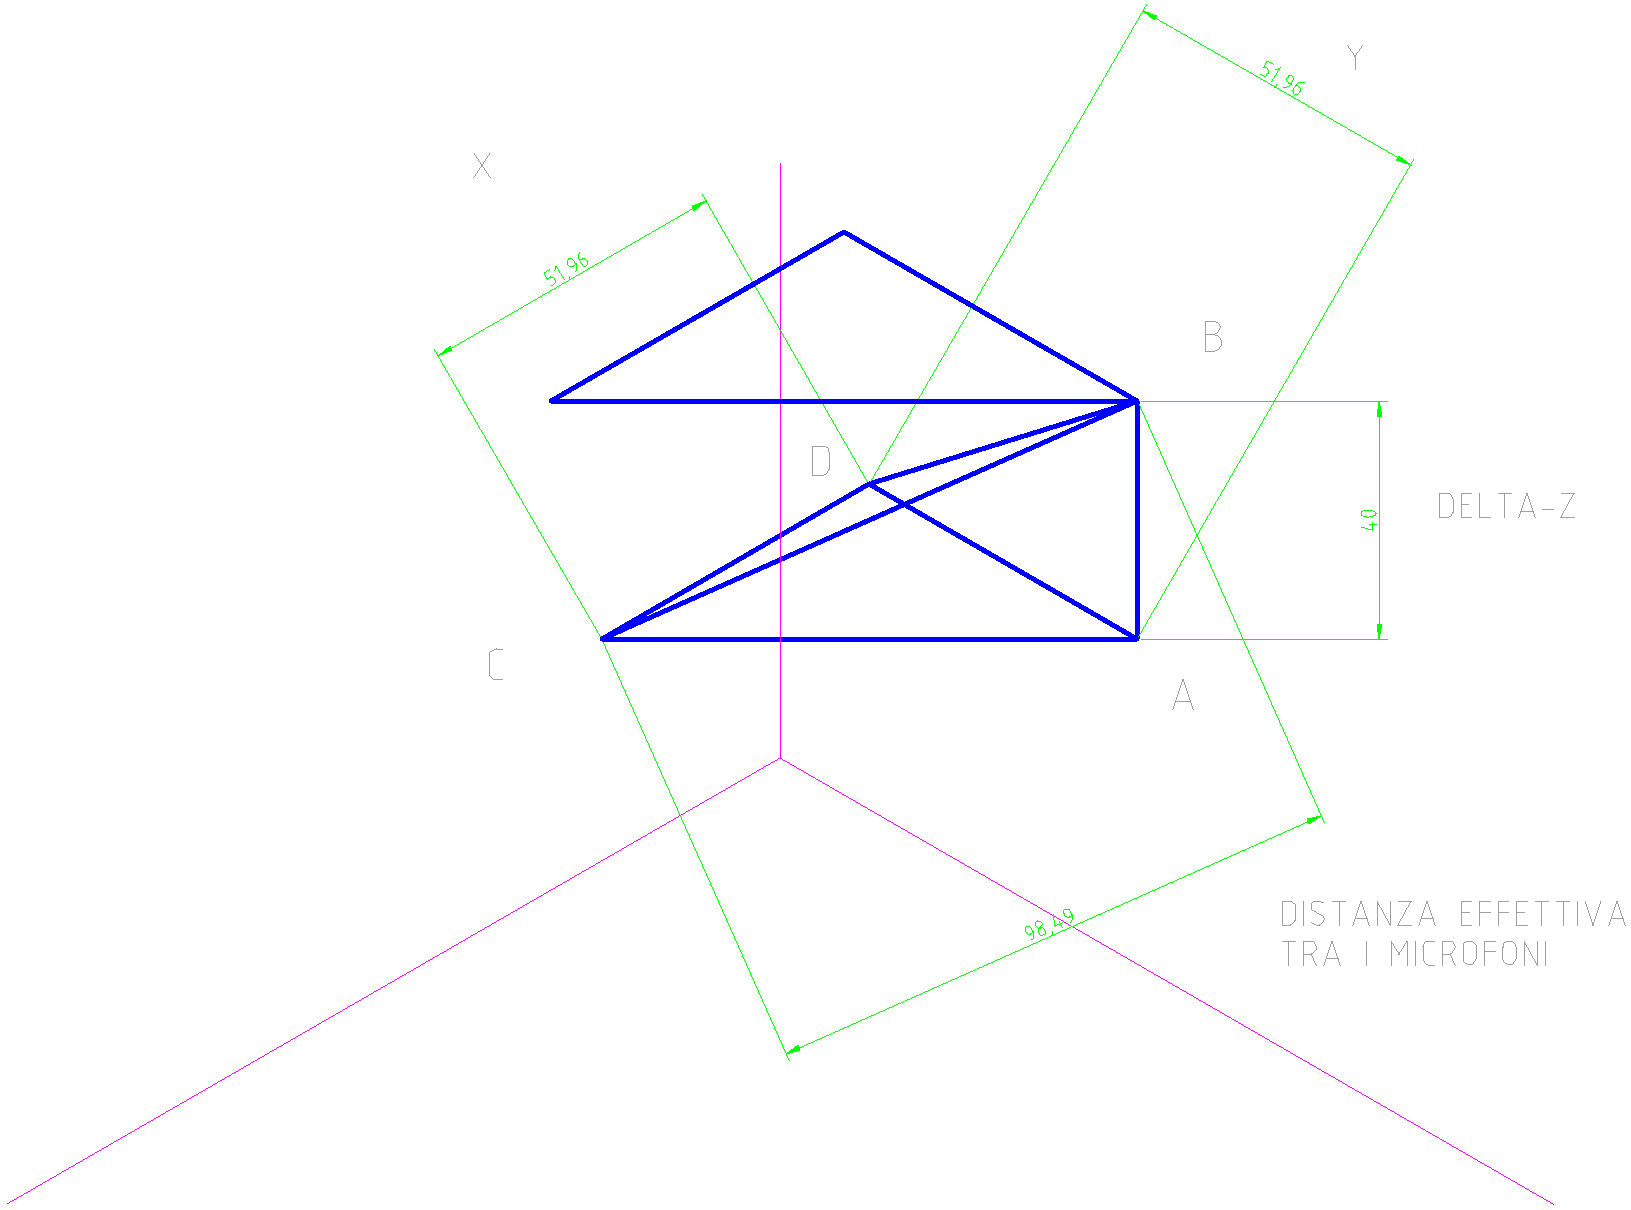
\includegraphics[width=0.7\textwidth]{images/Assonometria.png}
         \caption{\label{fig1}Assonometria}
    \end{figure}

    Per capire meglio la problematica, quindi, costruiamo una piramide a base triangolare, dove gli estremi contrassegnati con le lettere $B$ e $C$ rappresentano rispettivamente il centro della coppia spaziata e la posizione dello spot. Così facendo, nel nostro programma diamo in input le tre dimensioni $x, y, \Delta z$ che in termini geometrici saranno tradotte in
    $$x = CD$$
    $$y = DA$$
    $$z = AB$$
    Riusciamo quindi a calcolarci la distanza $CB$ attraverso l'applicazione del teorema di Pitagora.

    Per conoscere invece l'angolo di incidenza azimutale, ci serviamo dell'applicazione del teorema di Pitagora e del teorema del coseno
    $$BD = \sqrt{AD^2 + BA ^ 2}$$
    $$\widehat{CBD} = arccos \biggl( {CB ^ 2 + BD ^ 2 - CD ^ 2\over 2 * CB * BD} \biggr)$$

    Poiché il teorema di Pitagora e quello del coseno sono ricorrenti nelle funzioni che formalizzano il panner, dichiariamo una libreria apposita per tutte le funzioni matematiche denominandola ``11ts.lib'' e definendola così:
    
    \begin{lstlisting}
import("stdfaust.lib");
ts = library("12ts.lib");

//conversione da gradi a radianti e viceversa
deg2rad = * (ma.PI/180);
rad2deg = * (180/ma.PI);

//teorema di pitagora
pit(a,b) = sqrt(a ^ 2 + b ^ 2) : float;

//teorema di carnot per il calcolo dell'angolo compreso tra due lati. l1 e l2 sono i lati in cui è compreso l'angolo da calcolare, l3 è il lato opposto
acarnot(l1,l2,l3) = acos((l1 ^ 2 + l2 ^ 2 - l3 ^ 2)/(2 * l1 * l2)) : float;

//teorema di carnot per il calcolo del lato opposto ad un angolo già dato e i due contigui. l1 e l2 sono i lati, rad è l'angolo opposto
lcarnot(l1,l2,rad) = sqrt((l1^2) + ((l2^2) - 2*(l1) * (l2) * cos(rad))) : float;

//simulatore figura polare
ppattern(x,pp,inc) = ((1-pp) * x) + (pp * x * cos(inc));
    \end{lstlisting}
    
    
    In tale maniera costruiamo un codice pulito e riutilizzabile per qualsiasi nostro progetto.
    Difatti nel nostro progetto di Faust avremo la seguente situazione:
    
    \begin{lstlisting}
//OUTPUT DISTANZA REALE TRA I MICROFONI SULLE TRE COORDINATE
xyz2dst(cd,da,ab) = cb(ab,ca)
with{
    ca = ts.pit(cd,da);
    cb(ab,ca) = ts.pit(ab,ca);
};

//OUTPUT RADIANTI AZIMUT REALI
dst2arad(cd,da,ab) = arad(cb,db,cd,xsign)
with{
    cb = xyz2dst(cd,da,ab);

    xsign = cd : ma.signum;
    db = ts.pit(ab,da);
    arad(cb,db,cd,xsign) = ts.acarnot(cb,db,cd) : ts.rad2deg : _ * xsign : (_+90) : ts.deg2rad;
};
    \end{lstlisting}

    \subsection{La coppia main}
    
    Finora il main è stato considerato come un unico microfono, però, come ben chiaro, il progetto è finalizzato ad avere come main una coppia spaziata. Per comodità consideriamo ora la planimetria del progetto.

    \begin{figure}[H]
        \centering
        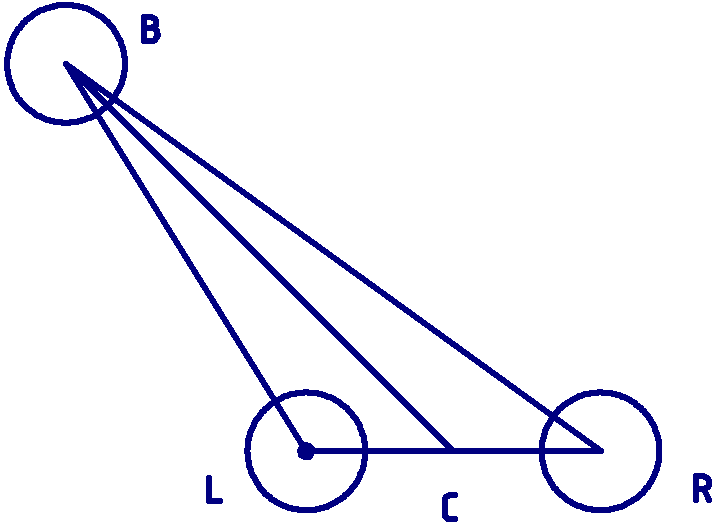
\includegraphics[width=0.5\textwidth]{images/PLANIMETRIA.png}
         \caption{\label{fig2}Planimetria}
    \end{figure}

    Conseguentemente il punto $C$ diventerà il centro della nostra coppia main. $CB$ quindi è la distanza tra il centro della coppia main e lo spot che vogliamo pannare.
    Ora è necessario effettuare tutti i calcoli trigonometrici per far si che L e R risultino due entità a parte. Questa operazione è il fulcro del nostro progetto, dato che ci permette di formalizzare, in seguito quella che è la vera differenza di fase, ampiezza e tempo tra il canale di sinistra e il canale di destra, in modo da effettuare un posizionamento nell'immagine stereofonica il più fedele possibile.
    Ora quindi richiamiamo le funzioni già adoperate in precedenza per calcolarci $LB$ e $RB$ \\
    
    \begin{lstlisting}
//DISTANZA REALE TRA CIASCUN MIC DELLA COPPIA MAIN E LA SORGENTE
dstmicmain(cd,da,ab,dst,rad) = dstsource(cb,dst,rad)
with{
    cb = xyz2dst(cd,da,ab);
    dstsource(cb,dst,rad) = ts.lcarnot(cb,dst/2,rad);
};
    \end{lstlisting}
    
    In tal maniera, definiamo la funzione $dstmicmain$ che richiameremo 2 volte: una per calcolare $LB$ e l'altra per calcolare $RB$.
    Come ben noto, la sorgente $B$ avrà un angolo di incidenza differente su $L$ e su $R$. Quindi dobbiamo calcolarci anche queste misure adoperando, come in precedenza, il teorema di Carnot.
    \footnote{Ad esempio: consideriamo $CB = 40 cm$, $LR = 20cm$ (quindi $LC=10cm$) e l'angolo $\widehat{BCR} = 135\textdegree$ (così come avviene nella planimetria della Fig. 2). L'angolo d'incidenza su $L$ sarà uguale a $122.88$ e su $R$ sarà $180-36.46=143.54$. Contando che l'orecchio umano è capace di percepire una differenza di un grado frontale - cosa che ovviamente non avviene nel cono di confusione, anche queste piccole differenze aiutano a percepire meglio l'effetto del nostro panner}
    
    \begin{lstlisting}
//ANGOLO DI INCIDENZA DELLA SORGENTE SU UNA CAPSULA
radmicmain(cd,da,ab,dst,rad) = inc(dst,dstcap,cb)
with{
    cb = xyz2dst(cd,da,ab);
    dstcap = dstmicmain(cd,da,ab,dst,rad);
    
    inc(dst,dstcap,cb) = ts.acarnot(dst/2,dstcap,cb) : ts.rad2deg : (90-_) : ts.deg2rad;
};
    \end{lstlisting}

    La parte dove si fa la differenza $(90-_)$ è fondamentale in quanto, matematicamente, la figura polare cardioide, nella sua definizione, è orientata sull'asse x. Quindi è necessario correggere l'angolo in base a questo dato.\\
\subsection{Il ritardo tra i due microfoni main}
    La velocità del suono influisce sulle differenze di tempo, quindi è necessario costruire una funzione che, prese in input le distanze tra la sorgente e ciascuna capsula microfonica, calcoli un ritardo attraverso un valore di velocità arbitrario, che in questo caso sarà $321 m/s$. La scelta non è casuale in quanto questo valore è uno standard utilizzato all'interno degli auditorium.

    \begin{lstlisting}
delaysig(sig,dst) = output(sig,delinsamples)
with {
    sspeed = 321;
    delinsamples = ((dst/100)/sspeed)*ma.SR : int;
    output(sig,delinsamples) = sig : de.sdelay(10000,256,delinsamples);
};
    \end{lstlisting}
    
\subsection{L'attenuazione}
    Altro dato importante è l'attenuazione del segnale in base alla distanza. Approssimativamente sappiamo che l'attenuazione è pari a 6 dB per ogni raddoppio della distanza. La nostra formula di attenuazione, ovviamente, è comunque approssimativa in quanto l'attenuazione non avviene linearmente per tutto lo spettro di frequenze della sorgente. Inoltre, la composizione dello spazio acustico e tutti i materiali influiscono molto sull'attenuazione. Poiché stiamo costruendo un modello matematico ideale, adoperiamo una formula di attenuazione che approssimi al meglio la resa sonora in un ambiente ideale. Nel nostro caso\\
    $$Att = \biggl({100 - 20*log_{10}(\frac{dst}{0.1})\over100} \biggr)$$
\begin{lstlisting}
att(sig,dst) = output(sig,dst)
with{
    //Leq=Lrif-20*Log10(r/rrif)
    output(sig,dst) = sig * (100 - 20*log10(dst/0.1))/100;
};
\end{lstlisting}

\subsection{Il panning e la funzione main}
Definiamo l'ultima funzione panner che ci permette di simulare la figura polare cardioide e omnidirezionale. 
\begin{lstlisting}
panner(sig,pp,inc) = pan(sig,pp,inc)
with {
    pan(sig,pp,inc) = ppattern(sig,pp,inc); 
};
\end{lstlisting}

Come ultima cosa racchiudiamo tutte le funzioni precedentemente definite in un'unica funzione main "multipanner".

\begin{lstlisting}
multipanner(sig,cd,da,ab,dst,dvg,pp) = l(sig,pp,totangleL,dstL), r(sig,pp,totangleR,dstR)
with{
    //radianti dal centro
    radL = dst2arad(cd,da,ab);
    radR = radL : rad2deg : (_-180) : deg2rad;

    incL = radmicmain(cd,da,ab,dst,radL) : rad2deg;
    incR = radmicmain(cd,da,ab,dst,radR) : rad2deg;

    dstL = dstmicmain(cd,da,ab,dst,radL);
    dstR = dstmicmain(cd,da,ab,dst,radR);

    totangleL = incL, dvg : + : deg2rad;
    totangleR = incR, dvg : + : deg2rad;

    l(sig,pp,totangleL,dstL) = panner(sig,pp,totangleL) : delaysig(_,dstL) : att(_,dstL);
    r(sig,pp,totangleR,dstR) = panner(sig,pp,totangleR) : delaysig(_,dstR) : att(_,dstR);
};

//process = multipanner; OGGETTO MAX
process = multipanner(_,cd, da, ab, dst, dvg, pp);
\end{lstlisting}
\section{Perché utilizzare il ``multipanner''}
    
    Un panner tradizionale LR ha come unica variabile la differenza d'ampiezza tra sinistra a destra. È facile intuire che questo potrebbe essere molto limitante in quanto non ci da una nessuna informazione stereofonica, o per lo meno che ci permette di effettuare un posizionamento nello spazio che riesca a far ``dialogare'' lo spot con la coppia main. Il panner oggetto di ricerca, invece, riesce a far comunicare lo spot con il main inserendo delle variabili spaziali. 
    Queste, rielaborate, ricostruiscono matematicamente parte di quello che succederebbe se riprendessimo la sorgente in quel determinato punto $[x, y, \Delta z]$ attraverso la coppia main. 
    Difatti nel nostro caso abbiamo provveduto non solo a differenziare l'ampiezza come avverrebbe con un panner LR, ma anche a fornire una differenza di tempo tra L e R e una spettrale. Così facendo ampliamo le possibilità di utilizzo del progetto che può anche essere utilizzato a fini creativi.

\section{Vantaggi e svantaggi}

\subsection{$x, y, \Delta z$}
    Lo strumento nasce per riprodurre nella maniera più fedele possibile la posizione di uno SPOT del panorama stereo prendendo come riferimento il main. Di conseguenza sarebbe opportuno approcciare a questo strumento in una maniera tale che il ``dialogo'' tra il MAIN e lo SPOT avvenga in maniera corretta.
    Durante la prima applicazione del panner nelle registrazioni orchestrali, non disponendo di misure precise di distanze $x, y, \Delta z$ , i risultati sono stati buoni, ma comunque con un margine di errore - nel nostro caso - trascurabile.
    Fatto sta che per ricavare tali misure è stato necessario non solo fare i rilievi delle distanze sul posto, ma anche fare un disegno tecnico della realtà di riferimento. Conseguentemente, in alcune situazioni potrebbe risultare scomodo utilizzare questo strumento se non si hanno degli adeguati strumenti di misurazione o delle adeguate competenze per fare un disegno tecnico. All'atto pratico la misurazione di  $x, y, \delta z$, però, è l'unico scoglio da superare nell'utilizzo del Multipanner. 

\subsection{La velocità del suono}
    Nel caso dell'utilizzo dei panner in un multitraccia di un'orchestra, uno dei vantaggi di avere dei delay su L e su R è quello di effettuare automaticamente l'allineamento di tutti i segnali degli spot verso la coppia main, evitando di effettuare il Ciak. Però c'è da considerare un problema: è abbastanza complesso rilevare la velocità del suono. Difatti noi nella definizione del multipanner, abbiamo utilizzato un valore convenzionale, nonché $321 m/s$ \footnote{La velocità del suono è variabile in base alla temperatura del luogo fisico dove viene emesso, all'umidità, alla pressione ecc. Ne consegue che in un ambiente più caldo e umido, ad esempio, il suono viaggia più velocemente, rendendo il valore di $321 m/s$ una mera approssimazione che potrebbe inficiare sulla qualità del risultato finale nell'applicazione dell'algoritmo qui proposto. Viceversa in un ambiente secco e freddo, il suono viaggia più lentamente, rendendo l'applicazione altrettanto fallace} . Per offrire una maggiore precisione allo strumento, sarebbe opportuno anche inserire una funzione di allineamento che rilevi automaticamente la velocità del suono nell'ambiente considerato - anche se non avremo mai una misura precisa al millesimo.
    
\subsection{Comb Filtering}
    Le differenze di tempo tra L e R fanno si che, nel caso della loro somma, ci siano fenomeni di comb filtering. Sarebbe quindi opportuno aggirare almeno parzialmente il problema lavorando a frequenze di campionamento più alte. Per evitare completamente il comb filtering, in una seconda versione, sarà integrata una parte di filtri allpass che correggono le cancellazioni di fase su tutto lo spettro.
\end{document}